\documentclass[sigconf,authorversion,nonacm]{acmart}

%%% Core packages (deduplicated for Overleaf stability) %%%
\usepackage{xurl}
\usepackage[belowskip=0pt,aboveskip=5pt]{subcaption}
\usepackage{listings}
\usepackage{enumitem}
\usepackage{booktabs}
\usepackage{xspace}
\usepackage{makecell}
\usepackage{amsmath}
\usepackage{amsthm}
\usepackage{pifont}
\usepackage{balance}
\usepackage{microtype}
\usepackage[ruled,vlined,linesnumbered]{algorithm2e}
\usepackage{comment}
\usepackage{adjustbox}
\usepackage{array,multirow,graphicx}
\newcommand{\DashboardScreenshot}{%
  \IfFileExists{FSM.png}{%
    \includegraphics[width=\linewidth,height=6.8cm,keepaspectratio]{FSM.png}%
  }{%
    \fbox{\parbox[c][6.8cm][c]{0.95\linewidth}{\centering\small\sffamily
        Missing \texttt{FSM.png} (dashboard screenshot). Place the file beside \texttt{report.tex} and rebuild.}}%
  }%
}
\usepackage{dblfloatfix}
\usepackage{float}
\usepackage{placeins}
\usepackage{tikz}
\usetikzlibrary{arrows.meta,positioning,fit,shapes.misc}
\usepackage{pgfplots}
\pgfplotsset{compat=1.18}
\setlength{\textfloatsep}{5pt plus 1pt minus 1pt}
\setlength{\floatsep}{5pt plus 1pt minus 1pt}
\setlength{\intextsep}{5pt plus 1pt minus 1pt}

%%% Code listings %%%
\definecolor{commentgreen}{rgb}{0,0.6,0}
\definecolor{codegray}{rgb}{0.5,0.5,0.5}
\definecolor{codepurple}{rgb}{0.58,0,0.82}
\lstdefinestyle{code}{
  backgroundcolor=\color{gray!4},
  commentstyle=\color{commentgreen},
  keywordstyle=\color{codepurple},
  numberstyle=\tiny\color{codegray},
  stringstyle=\color{codegray},
  basicstyle=\ttfamily\footnotesize,
  breaklines=true,
  captionpos=b,
  keepspaces=true,
  numbers=left,
  numbersep=5pt,
  showstringspaces=false,
  tabsize=2,
}
\lstset{style=code}

\SetKwInput{KwInput}{Input}
\SetKwInput{KwOutput}{Output}

\begin{document}

\title{CS 527 Research Project Report: Group 12}


\author{David Zhao, Chelsea Sun}
\affiliation{
    \institution{University of Illinois at Urbana-Champaign}
}
\email{[dekaiz2,qiaochu9]@illinois.edu}

\begin{abstract}
Intermittent faults are routine in deployed software; encoding explicit failure/recovery lifecycles supports regression testing and auditability. Our team presents a compact, model-driven fault-tolerant \emph{controller} as a three-state finite-state machine (\emph{Operational}/\emph{Error}/\emph{Recovery}) that drives \emph{real} local injections and repairs (TCP, SQLite, worker queue), with ``recovered'' treated as a falsifiable claim via handler-specific post-conditions. Concretely, \emph{FaultTolerantSystem} (\emph{state\_machine.py}) coordinates handlers under locks, a Flask dashboard exposes status and lab-aligned knobs, and \emph{run\_simulation.py} evaluates a $4{\times}3$ environment grid with $N{=}100$ trials per cell on a long-lived instance, exporting \emph{simulation\_results.csv} and \emph{simulation\_summary.csv}. In our archived run ($n{=}1200$), single-shot recovery succeeds in \textbf{every} trial---an outcome we engineered toward (deterministic repairs + checks), not a universal real-world theorem. Latency spans orders of magnitude: idle TCP/worker paths are sub-second versus multi-second paths under synthetic CPU stress (SQLite is the outlier), with an $\approx$100\,ms mean shift when a pre-recovery network delay knob is enabled.
\end{abstract}

\maketitle
\raggedbottom

\section{Introduction}
Fault tolerance remains central for systems operating under partial synchrony, shared infrastructure, and operational churn. A standard engineering pattern is to elevate recovery to a \emph{first-class} lifecycle: detect degradation, enter a controlled recovery mode, and return to service with evidence-backed checks rather than informal assurances.

Our team studies a deliberately scoped instantiation: a discrete \emph{controller} coupled to small but \emph{real} local subsystems (sockets, files, threads) that we injectively break and then repair. Conceptually, this sits in the same \emph{experimental resilience} tradition as recent software-engineering work on controlled fault injection and chaos-style evaluation~\cite{owotogbe2024chaos,he2024microfi}, but we deliberately keep the surface area small (local OS resources and an explicit FSM) rather than industrial-scale microservice meshes. At course-project scale we do \emph{not} model a full distributed stack; instead, we separate (i)~\emph{lifecycle policy}---when to enter \textbf{Error}, when to call \emph{attempt\_recovery}, how to record metrics---from (ii)~\emph{subsystem mechanics} in per-type handlers. Recovery success is decided by handler verification (I/O and computation), not by a synthetic Bernoulli draw in the harness. A background \emph{recovery watch} retries \emph{attempt\_recovery} only from \textbf{Error} with backoff and does \emph{not} inject new faults.

\paragraph{Problem and motivation.}
Interleaving fault logic with business logic complicates reasoning and testing. Model-based thinking encourages an explicit controller for lifecycle transitions; our artifact instantiates that separation with an FSM, concrete handlers, and a thin Flask observability layer.

\paragraph{Contributions.}
Our team contributes: \textbf{(i)}~a documented three-state FSM with per-\emph{FaultType} routing and metrics; \textbf{(ii)}~a reference Python implementation (\emph{state\_machine.py}, \emph{faults/}) with locks, optional stress/delay knobs aligned to the harness, and imperative APIs (\emph{trigger\_fault}, \emph{attempt\_recovery}, \emph{set\_recovery\_env}); \textbf{(iii)}~a dashboard (\emph{app.py}, \emph{templates/index.html}) plus \textbf{(iv)}~a batch harness (\emph{run\_simulation.py}) that sweeps four environment cells on a long-lived \emph{FaultTolerantSystem} and exports CSVs; and \textbf{(v)}~tests (\emph{tests/test\_state\_machine.py}) intended to encode behavioral contracts as the API stabilizes.


\section{Approach Overview}
\label{sec:overview}
We frame fault tolerance as \emph{closed-loop control} on a discrete state space with transitions tied to real local effects. The controller begins in \textbf{Operational}; \emph{trigger\_fault} moves us to \textbf{Error} via a handler-chosen break, and \emph{attempt\_recovery} enters \textbf{Recovery} while \emph{try\_recover()} runs; handler verification (not a random simulator coin-flip) decides success, returning to \textbf{Operational} or \textbf{Error} for backoff retries. This thin policy shell in \emph{FaultTolerantSystem} supports two validation modes that our team actually used day-to-day: interactive dashboard runs and CSV-backed batch sweeps from \emph{run\_simulation.py}.

\section{Approach Details}
\label{sec:details}

\subsection{End-to-end architecture}
Our team's codebase stacks five layers: \textbf{(model)}~\emph{FaultTolerantSystem} in \emph{state\_machine.py}; \textbf{(handlers)}~\emph{faults/} with \emph{trigger\_fault}/\emph{try\_recover}; \textbf{(service)}~Flask routes in \emph{app.py} (\emph{/api/inject\_fault}, \emph{/api/recovery\_env}, reset); \textbf{(UI)}~\emph{templates/index.html} polling \emph{/api/status}; and \textbf{(eval)}~\emph{run\_simulation.py} exporting \emph{simulation\_results.csv} and \emph{simulation\_summary.csv}.

\subsection{Examples to explain the approach}

\paragraph{Finite-state contract (figure).}
Let $S=\{\textsc{Op},\textsc{Err},\textsc{Rec}\}$ and enumerate three labels (\emph{FaultType}) with dedicated handler instances. The controller remains a thin dispatcher: it enforces admissible transitions (e.g., new faults only from \textsc{Op}) while repair specifics live in handlers whose probes differ (TCP, SQLite, worker). Figure~\ref{fig:fsm} states the contract; expensive handler work runs under \textsc{Rec} outside the lock so readers are not blocked.

\begin{figure}[!ht]
  \centering
  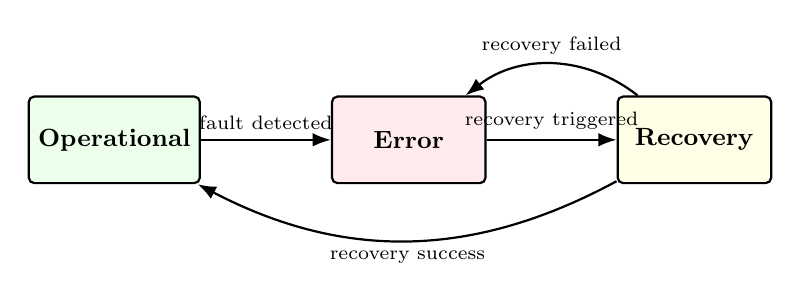
\begin{tikzpicture}[
    >=Latex,
    node distance=1.65cm,
    every node/.style={font=\small},
    st/.style={draw, rounded corners=2pt, minimum width=1.95cm, minimum height=1.1cm, align=center, thick},
  ]
    \node[st, fill=green!8] (op) {\textbf{Operational}};
    \node[st, fill=red!8, right=of op] (err) {\textbf{Error}};
    \node[st, fill=yellow!10, right=of err] (rec) {\textbf{Recovery}};
    \draw[->, thick] (op) -- node[above, font=\scriptsize] {fault detected} (err);
    \draw[->, thick] (err) -- node[above, font=\scriptsize] {recovery triggered} (rec);
    \draw[->, thick] (rec) to[bend left=28] node[below, font=\scriptsize] {recovery success} (op);
    \draw[->, thick] (rec) to[bend right=38] node[above, font=\scriptsize] {recovery failed} (err);
  \end{tikzpicture}
  \caption{Finite state machine used by our fault-tolerant controller. Separately, a background \emph{recovery watch} thread may invoke \emph{attempt\_recovery} again whenever the controller is stuck in \textbf{Error} (fixed backoff between tries); it does not inject new faults.}
  \label{fig:fsm}
\end{figure}

\paragraph{Imperative kernel (code listings).}
Listings~\ref{lst:trigger}--\ref{lst:recover} show the guarded kernel: faults are accepted only in \textsc{Op} under a lock; recovery flips to \textsc{Rec}, copies handler pointers, then performs I/O \emph{outside} the lock before re-entering to commit metrics/state.

\begin{lstlisting}[language=Python, basicstyle=\ttfamily\scriptsize, caption={\emph{trigger\_fault} (excerpt).}, label={lst:trigger}]
def trigger_fault(self, fault_type):
    with self._lock:
        if self.state != State.OPERATIONAL:
            return False
        handler = self._handlers[fault_type]
        handler.trigger_fault()
        self.state = State.ERROR
        self._current_fault_type = fault_type
        self._current_handler = handler
        self.metrics["total_faults"] += 1
        return True
\end{lstlisting}

\begin{lstlisting}[language=Python, basicstyle=\ttfamily\scriptsize, caption={\emph{attempt\_recovery} (excerpt; lock released before I/O).}, label={lst:recover}]
def attempt_recovery(self):
    with self._lock:
        if self.state != State.ERROR:
            return False, "Not in error state"
        self.state = State.RECOVERY
        handler = self._current_handler
        ftype = self._current_fault_type
        use_stress = self.web_stress_recovery
        net_delay_ms = self.web_net_delay_ms
    if ftype == FaultType.NETWORK_TIMEOUT and net_delay_ms > 0:
        time.sleep(net_delay_ms / 1000.0)
    if use_stress:
        with _stress_load():
            success, message = handler.try_recover()
    else:
        success, message = handler.try_recover()
    with self._lock:
        if success:
            self.metrics["successful_recoveries"] += 1
            self.state = State.OPERATIONAL
            # ... metrics, logging, clear current handler ...
        else:
            self.metrics["failed_recoveries"] += 1
            self.state = State.ERROR
    return success, message
\end{lstlisting}

\noindent Recent fault-injection and resilience work likewise foregrounds \emph{instrumented} campaigns and recovery semantics that can be checked against real subsystem behavior rather than synthetic randomness~\cite{he2024microfi,assad2024icse}. Listings~\ref{lst:trigger}--\ref{lst:recover} are the concrete locus of that stance in our artifact: ``recovered'' is decided by handler probes and I/O effects, not by a Bernoulli draw in the harness.

\paragraph{Monitoring dashboard.}
See Figure~\ref{fig:dash}. The dashboard and recovery-watch both call the model, so our team serializes bookkeeping with a lock and keeps slow handler work out of the critical section. The live UI (\emph{app.py}, \emph{templates/index.html}) fetches \emph{/api/status}, supports inject-then-recover and reset, and exposes the same \emph{web\_stress\_recovery} / \emph{web\_net\_delay\_ms} fields as the batch harness (this saved us from printf-only debugging).

Automated tests (\emph{tests/test\_state\_machine.py}) are intended to encode behavioral contracts for the FSM; when the test API matches the imperative kernel, they support the rubric goal of \emph{methodological rigor}.

\subsection{Algorithms for systematic presentation or approach (50 pts)}
Algorithm~\ref{alg:autostep} sketches \emph{\_auto\_step}: from \textsc{Err}, wait backoff $\Delta{=}0.5$\,s then call \emph{attempt\_recovery} (no autonomous fault sampling). Algorithm~\ref{alg:trial} summarizes one batch trial on a long-lived controller: time one inject+recover pair, optionally under CPU stress (eight threads via \texttt{stress\_load}), inserting \emph{sleep}($d/1000$) before \emph{attempt\_recovery} only for the network fault when $d{>}0$, in the same order as the inner \texttt{inject\_and\_recover} closure in \emph{run\_simulation.py}.

\paragraph{Implementation notes.}
The pseudocode is meant to track the main branches in \emph{state\_machine.py} and \emph{run\_simulation.py} without reproducing every field in the returned row. Concretely, \texttt{\_auto\_step} only sleeps and calls \emph{attempt\_recovery} from \textsc{Err}; the watch loop is \texttt{start\_auto(interval)} (\texttt{\_auto\_step} then sleep \texttt{interval}). Our Flask entry point passes \texttt{RECOVERY\_WATCH\_INTERVAL\_S}${=}2.0$\,s, while the Python default for \texttt{interval} is still \texttt{4.0}\,s if a caller omits it. Algorithm~\ref{alg:trial} compresses the trial payload as $(ok,\Delta t,msg)$; the implementation records a richer dict (\texttt{recovered}, \texttt{time\_s}, \texttt{message}, \ldots). The inject path is \texttt{trigger\_fault} $\rightarrow$ optional \texttt{time.sleep} for network+$d{>}0$ $\rightarrow$ \texttt{attempt\_recovery}.

\begin{algorithm}[!t]
\caption{Recovery-watch timestep (\emph{\_auto\_step})}
\label{alg:autostep}
\KwInput{Controller with state $\sigma$}
\KwOutput{Side effects on subsystem handlers and updated $\sigma$}
\If{$\sigma = \textsc{Err}$}{
  Wait fixed backoff $\Delta$ (e.g., 0.5\,s)\;
  \emph{attempt\_recovery}() \tcp*{$\sigma$ ends in \textsc{Op} or \textsc{Err}}
}
\KwRet{}\;
\end{algorithm}

\begin{algorithm}[!t]
\caption{Single batch evaluation trial (environment-aware)}
\label{alg:trial}
\KwInput{Controller $C$, fault type $f$, stress flag $s$, network delay $d$ (ms)}
\KwOutput{Boolean recovered flag, elapsed wall time, diagnostic message}
\lIf{$C.\sigma \neq \textsc{Op}$}{\KwRet{skip}}
$t_0 \leftarrow$ wall clock\;
\If{$s$}{\textbf{with} CPU stress threads \textbf{do} \emph{inject\_and\_recover}($C,f,d$)\;}
\Else{\emph{inject\_and\_recover}($C,f,d$)\;}
$t_1 \leftarrow$ wall clock\;
\KwRet{$(\textit{ok},\, t_1{-}t_0,\, \textit{msg})$}\;
\end{algorithm}
\noindent \emph{inject\_and\_recover} expands to \emph{trigger\_fault}($f$); optional network delay sleep; \emph{attempt\_recovery}(). That ordering is what \emph{run\_simulation.py} logs as wall-clock \emph{time\_s}. In our artifact, ``recovered'' is what handler probes report after real I/O, not a synthetic coin flip in the harness.

\section{Experimental Evaluation}
\label{sec:eval}
We evaluate \emph{functional correctness} under a scripted inject+recover protocol and \emph{observability} via CSV exports plus the dashboard. Section~\ref{sec:plan} states what our team sweeps and logs (with RQs); Section~\ref{sec:results} revisits those questions with the summary table, plots grouped by topic, and a brief synthesis on mechanisms and limits.

\section{Evaluation Plan}
\label{sec:plan}
\paragraph{Environment grid and protocol.}
Our team sweeps \emph{EnvConfig.default\_grid}: (\emph{idle\_d0}, \emph{idle\_d100}, \emph{stress\_d0}, \emph{stress\_d100}). \emph{stress} wraps inject+recover with eight CPU-bound threads; \emph{d100} inserts an extra 100\,ms sleep before recovery \emph{only} for the network fault (database/server ignore $d$). For each $(e,f)$ we allocate one long-lived \emph{FaultTolerantSystem}, run $N{=}100$ trials (\emph{run\_block}; first trial \emph{cold\_start}), log \emph{recovered}, \emph{time\_s}, and session metadata, and export $4{\times}3{\times}100=1200$ rows to \emph{simulation\_results.csv}. \emph{run\_simulation.py} aggregates cohort means/variance/P50/P95, plus \emph{cold\_only}, \emph{warm\_only}, and \emph{success\_rate\_pct}, into \emph{simulation\_summary.csv}.

\paragraph{Reproducibility.}
Re-run: {\footnotesize\texttt{python run\_simulation.py --trials 100 --output simulation\_results.csv --summary simulation\_summary.csv}}. Timings vary with OS scheduling, Windows SQLite locking, and load; Table~\ref{tab:grid} and the figures use one completed archive attached to this report.

\subsection{Research questions}
Our measurements are organized around the following questions:
\begin{itemize}[leftmargin=*,nosep]
  \item \textbf{RQ1 (Knob isolation / harness wiring):} Do cohort statistics behave as the code promises---e.g., does the injected pre-recovery delay move only the network fault row while database and server means stay flat across \emph{d0} vs.\ \emph{d100}, matching the conditional \texttt{sleep} in \emph{run\_simulation.py}?
  \item \textbf{RQ2 (Latency by fault class and environment):} How do wall-clock recovery times differ across network, database, and worker-crash handlers under idle versus CPU-stressed recovery, and with versus without an extra 100\,ms delay before network recovery?
  \item \textbf{RQ3 (Cold vs.\ warm sessions):} On a long-lived controller, does the first trial in a block (cold start) differ materially from subsequent trials (warm) in mean latency or variance?
  \item \textbf{RQ4 (Dashboard vs.\ harness parity):} Do the Flask lab knobs (\emph{/api/recovery\_env}) expose the same controller fields and handler paths as the batch harness, so interactive debugging stays faithful to the code evaluated in CSV sweeps (with documented differences in how CPU stress is scoped in wall-clock time)?
\end{itemize}

\section{Evaluation Results and Discussion}
\label{sec:results}
Section~\ref{sec:plan} motivates the sweep; here we revisit the same questions with Table~\ref{tab:grid} as the shared numeric backbone. A short synthesis at the end connects the patterns and revisits the archived sweep in that light.

\begin{table*}[t]
  \centering
  \caption{Mean / P50 / P95 recovery time (seconds) per environment configuration and fault type. Rows group by \emph{config\_id}; statistics come from \emph{simulation\_summary.csv} (successful trials only).}
  \label{tab:grid}
  \small
  \setlength{\tabcolsep}{4pt}
  \begin{tabular}{@{}l l r r r@{}}
    \toprule
    \emph{config\_id} & Fault type & mean & P50 & P95 \\
    \midrule
    \emph{idle\_d0}   & Network Timeout   & 0.812 & 0.812 & 0.827 \\
    \emph{idle\_d0}   & Database Failure & 0.0107 & 0.0102 & 0.0126 \\
    \emph{idle\_d0}   & Server Crash      & 0.708 & 0.706 & 0.716 \\
    \emph{idle\_d100} & Network Timeout   & 0.911 & 0.909 & 0.926 \\
    \emph{idle\_d100} & Database Failure & 0.00958 & 0.00903 & 0.0121 \\
    \emph{idle\_d100} & Server Crash      & 0.708 & 0.708 & 0.716 \\
    \emph{stress\_d0} & Network Timeout   & 4.88 & 4.79 & 6.34 \\
    \emph{stress\_d0} & Database Failure & 9.09 & 9.01 & 11.4 \\
    \emph{stress\_d0} & Server Crash      & 3.21 & 3.24 & 4.40 \\
    \emph{stress\_d100} & Network Timeout   & 6.20 & 6.25 & 7.90 \\
    \emph{stress\_d100} & Database Failure & 9.52 & 9.49 & 11.6 \\
    \emph{stress\_d100} & Server Crash      & 3.29 & 3.25 & 4.53 \\
    \bottomrule
  \end{tabular}
\end{table*}

\subsection{RQ1: Knob isolation / harness wiring}
The batch harness wires the delay knob only on the \texttt{NETWORK\_TIMEOUT} path (see Algorithm~\ref{alg:trial} and \emph{run\_simulation.py}). Table~\ref{tab:grid} already supports that story qualitatively: moving from \emph{d0} to \emph{d100} adds $\approx$0.10\,s to the network row at \emph{idle} and further separates the network row under \emph{stress}, while database and server means stay in the same bands across \emph{d0}/\emph{d100} (modulo micro-jitter from scheduling). Figure~\ref{fig:delayknob} makes the same contrast explicit as mean deltas \emph{d100}$-$\emph{d0} per fault type under idle and stress: the network bar sits near the intended $+0.10$\,s band, whereas the other faults hug zero. Taken together, this is evidence that our cohort statistics are attributable to the documented conditionals rather than accidental cross-talk between fault labels.

\begin{figure*}[!tp]
  \centering
  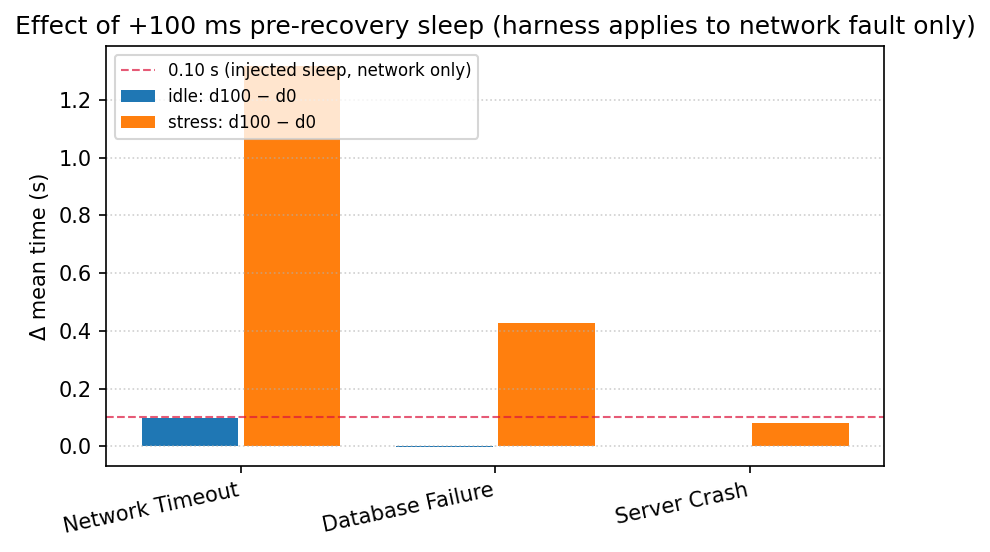
\includegraphics[width=\linewidth,height=4.4cm,keepaspectratio]{plot_delay_knob_delta.png}
  \caption{Mean increase from \emph{d0} to \emph{d100} cells (idle vs.\ stress), by fault type (RQ1: delay knob isolation).}
  \label{fig:delayknob}
\end{figure*}

\subsection{RQ2: Latency by fault class and environment}
Table~\ref{tab:grid} is the primary quantitative view: means, medians, and P95s for each $(\emph{config\_id}, \text{fault})$ cell. Stress inflates every fault row relative to idle; SQLite becomes the dominant cost center under \emph{stress\_*} (means near $\approx$9--9.5\,s), while TCP and worker paths move into multi-second bands but remain well below the database ceiling. Figure~\ref{fig:latency} is an \emph{idle\_d0} sanity check on a log axis: if centisecond-scale SQLite work ever inverted above $\sim$0.7--0.9\,s TCP/worker verification, our team would treat it as a wiring bug, not a brag. Figures~\ref{fig:hm} and \ref{fig:line} summarize the full $4{\times}3$ mean layout and how means move along \emph{idle\_d0}$\rightarrow$\emph{idle\_d100}$\rightarrow$\emph{stress\_d0}$\rightarrow$\emph{stress\_d100}. Figure~\ref{fig:stressup} plots $\mathbb{E}[T\mid\text{\emph{stress}}]-\mathbb{E}[T\mid\text{\emph{idle}}]$ per fault for \emph{d0}/\emph{d100}; Figure~\ref{fig:meanbar} adds mean$\pm$ sample standard deviation bars; Figure~\ref{fig:boxenv} exposes tails and IQR that scalar means hide.

\begin{figure}[!t]
  \centering
  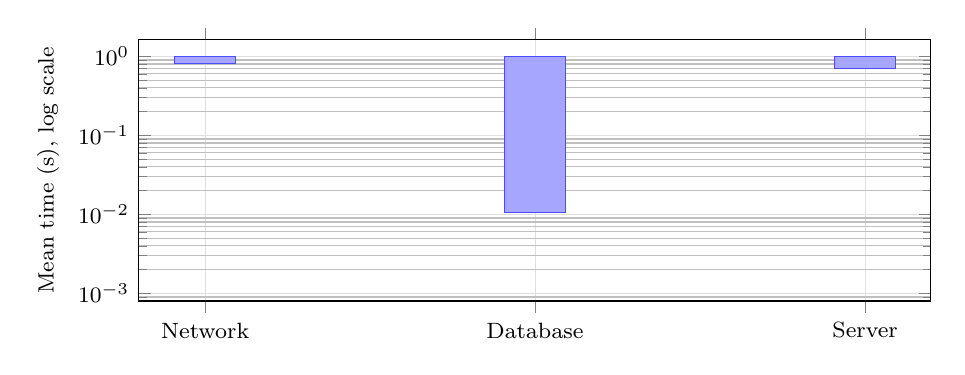
\begin{tikzpicture}
    \begin{axis}[
      ybar,
      width=0.96\linewidth,
      height=4.9cm,
      ymin=0.0008,
      ymode=log,
      log basis y={10},
      ylabel={Mean time (s), log scale},
      symbolic x coords={Network,Database,Server},
      xtick=data,
      x tick label style={font=\footnotesize, text width=1.6cm, align=center},
      y tick label style={font=\footnotesize},
      label style={font=\footnotesize},
      bar width=22pt,
      grid=both,
      major grid style={line width=.08pt, draw=gray!25},
    ]
      \addplot[fill=blue!35, draw=blue!70] coordinates {
        (Network,0.812368)
        (Database,0.01068)
        (Server,0.708035)
      };
    \end{axis}
  \end{tikzpicture}
  \caption{Mean successful recovery time by fault type for \emph{idle\_d0} ($n{=}100$). Log scale emphasizes the gap between SQLite work (centiseconds) and TCP/worker paths ($\sim$0.7--0.8\,s) absent stress or injected network delay.}
  \label{fig:latency}
\end{figure}

\begin{figure*}[!tp]
  \centering
  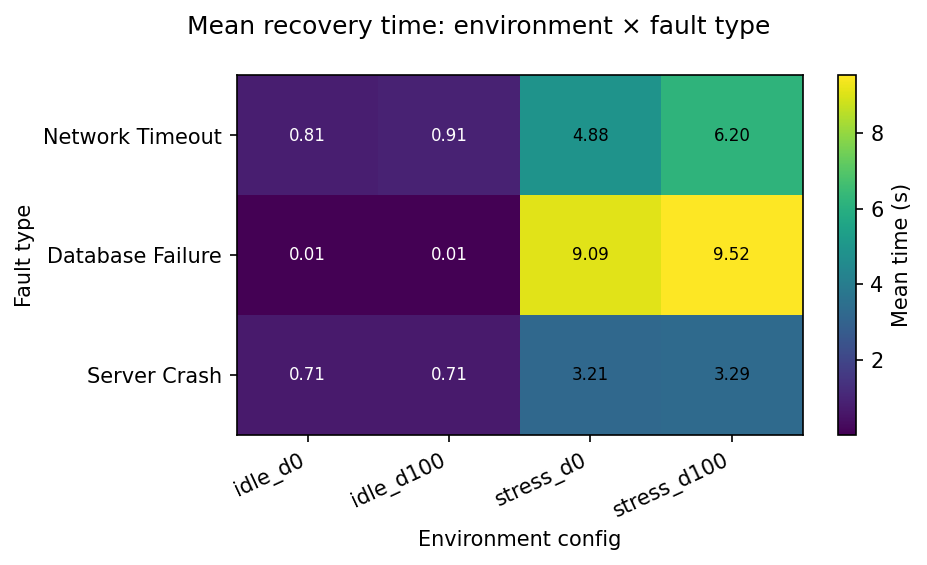
\includegraphics[width=\linewidth,height=4.5cm,keepaspectratio]{plot_mean_heatmap.png}
  \caption{Mean recovery time heatmap (fault type $\times$ \emph{config\_id}), $n{=}100$ per cell.}
  \label{fig:hm}
\end{figure*}

\begin{figure*}[!tp]
  \centering
  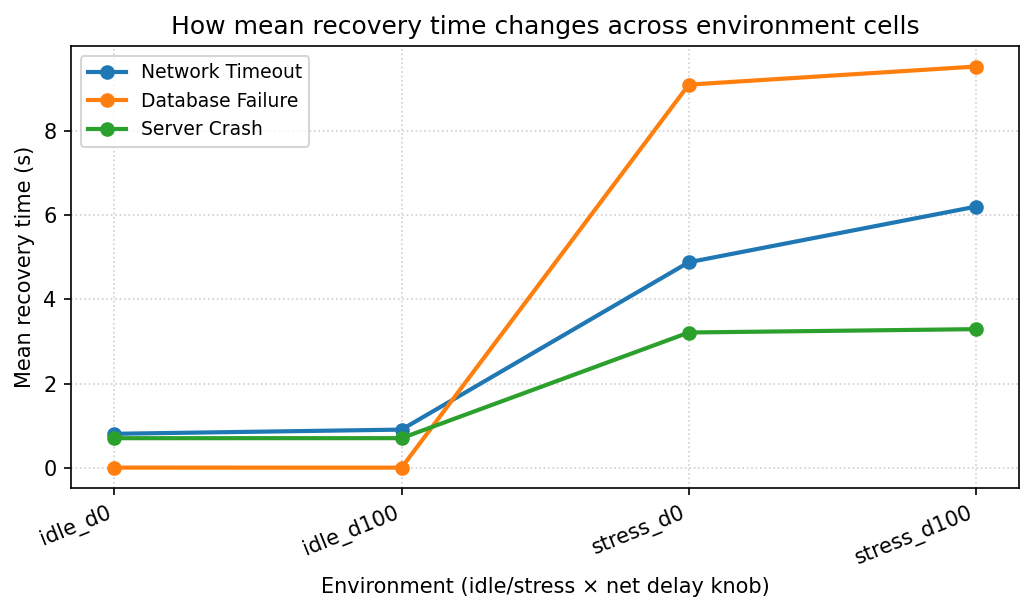
\includegraphics[width=\linewidth,height=4.5cm,keepaspectratio]{plot_mean_line_by_env.png}
  \caption{Mean recovery time vs.\ environment cell (one series per fault type), $n{=}100$ per cell.}
  \label{fig:line}
\end{figure*}

\begin{figure*}[!tp]
  \centering
  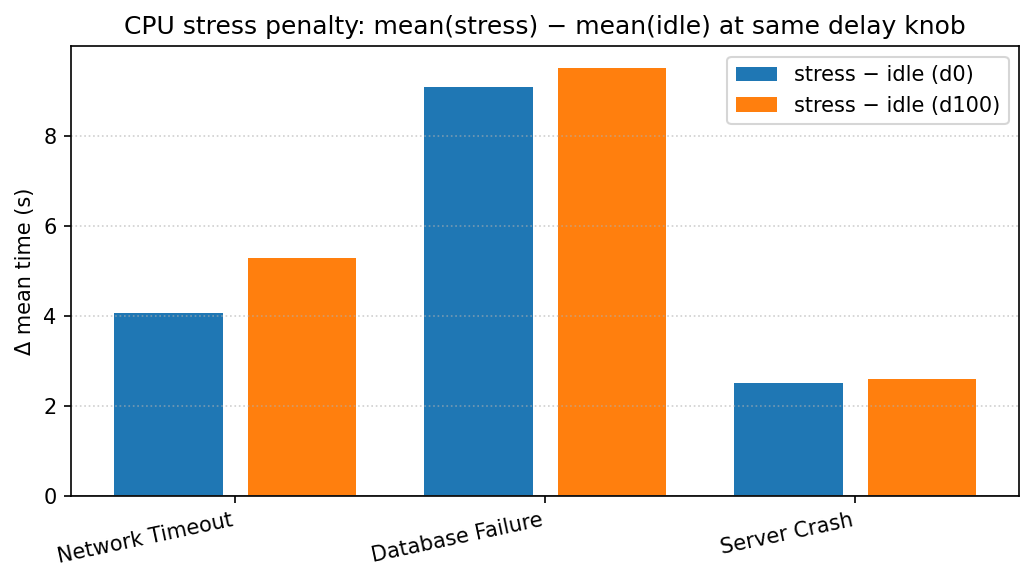
\includegraphics[width=\linewidth,height=4.5cm,keepaspectratio]{plot_stress_uplift.png}
  \caption{Stress penalty: mean recovery time under \emph{stress} minus mean under \emph{idle}, shown separately for \emph{d0} and \emph{d100}.}
  \label{fig:stressup}
\end{figure*}

\begin{figure*}[!tp]
  \centering
  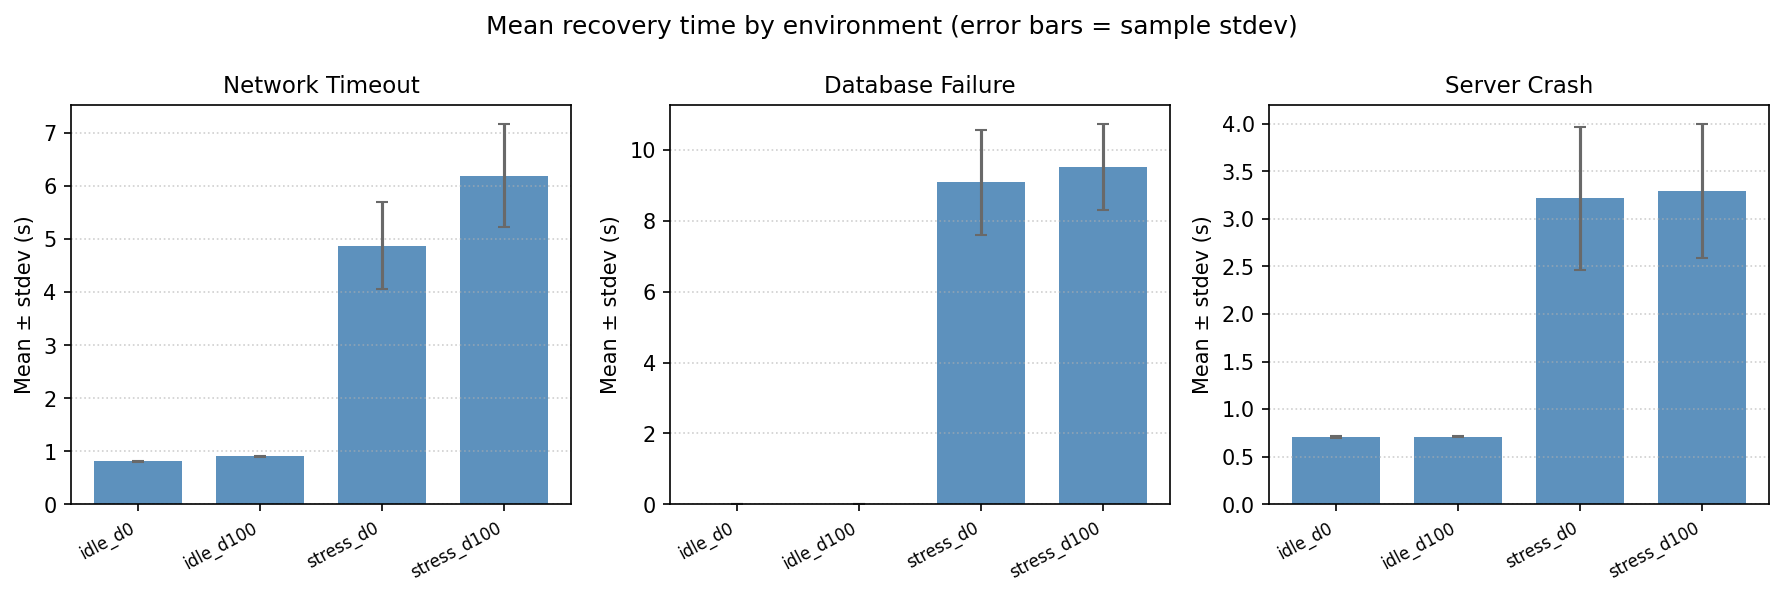
\includegraphics[width=\linewidth,height=4.5cm,keepaspectratio]{plot_mean_bar_by_fault.png}
  \caption{Mean$\pm$ sample standard deviation of recovery time for each \emph{config\_id}, split by fault type (panel).}
  \label{fig:meanbar}
\end{figure*}

\begin{figure*}[!tp]
  \centering
  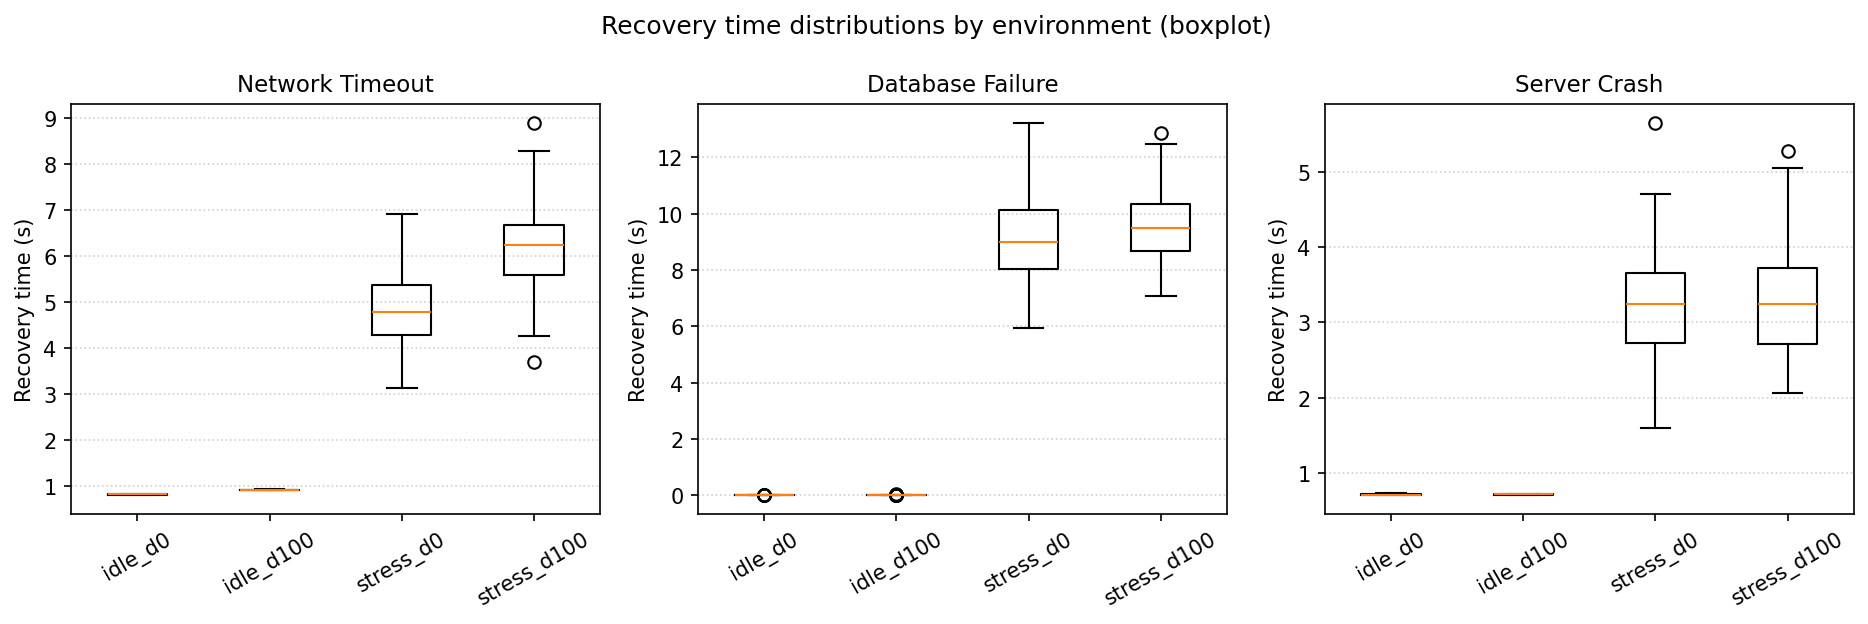
\includegraphics[width=\linewidth,height=4.5cm,keepaspectratio]{plot_recovery_box_by_fault.png}
  \caption{Recovery time distributions by fault type and environment (boxplot).}
  \label{fig:boxenv}
\end{figure*}

\subsection{RQ3: Cold vs.\ warm sessions}
Each $(\emph{config\_id}, \text{fault})$ block keeps one long-lived controller; the first trial in a block is tagged \emph{cold\_start} and later trials are warm. Figure~\ref{fig:coldwarm} pools all environment cells to show first-trial vs.\ later-trial means side by side. The companion CSV (\emph{simulation\_summary.csv}) carries the same split as numeric \emph{cold\_only} / \emph{warm\_only} rows without duplicating them as extra plots here; we use those rows when we want variance or P95 contrasts that the pooled figure de-emphasizes.

\begin{figure*}[!tp]
  \centering
  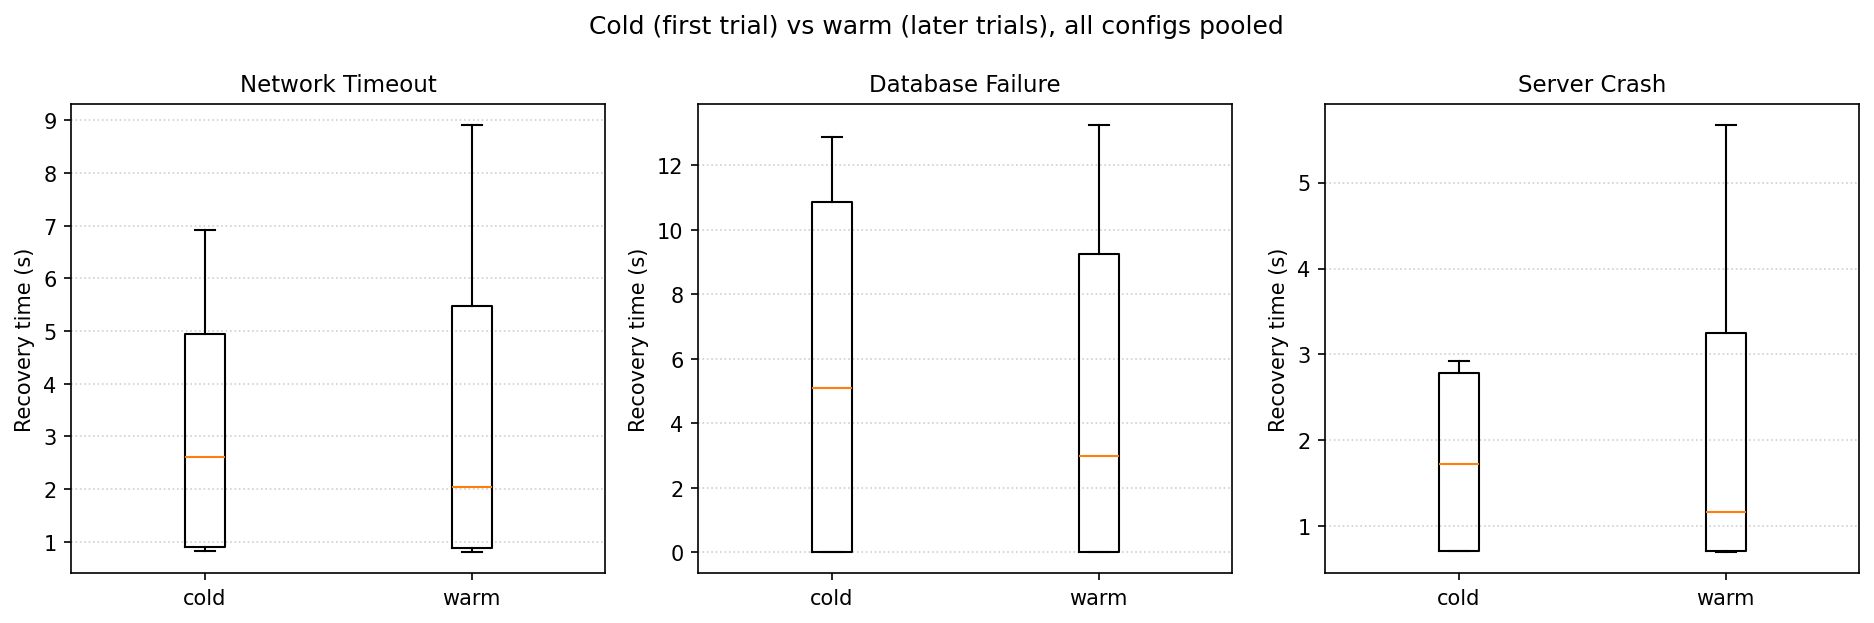
\includegraphics[width=\linewidth,height=4.5cm,keepaspectratio]{plot_recovery_cold_vs_warm.png}
  \caption{Cold vs.\ warm trials (all configs pooled), by fault type.}
  \label{fig:coldwarm}
\end{figure*}

\subsection{RQ4: Dashboard vs.\ harness parity}
The batch harness does not call \emph{set\_recovery\_env}; it passes \texttt{stress} and \texttt{net\_delay\_ms} into \emph{run\_trial}, which (i)~wraps the whole \texttt{inject\_and\_recover} closure in \texttt{stress\_load} when the profile is \emph{stress\_*}, and (ii)~sleeps $d/1000$ before \emph{attempt\_recovery} only for the network fault. The Flask route \emph{/api/recovery\_env} instead writes the same \emph{semantic} knobs into the controller (\emph{web\_stress\_recovery}, \emph{web\_net\_delay\_ms}) that \emph{attempt\_recovery} already reads---so interactive runs exercise the same handler code paths, with one documented nuance: UI stress wraps mainly \texttt{try\_recover}, whereas the CSV sweep's stress context spans fault injection plus recovery, so wall-clock seconds are not guaranteed to match click-for-click. For the archived grid we treat CSV as authoritative; the dashboard is how our team sanity-checked state transitions, metrics, and knob wiring before trusting sweeps. Figure~\ref{fig:dash} is the live \emph{/api/status} view (recent log lines, metrics, and lab controls); a small client-side replay smooths races between UI polling and fast transitions.

\begin{figure}[!ht]
  \centering
  \DashboardScreenshot
  \caption{Live monitoring dashboard (RQ4). The UI fetches \emph{/api/status} on demand, supports inject-then-recover and reset, optional lab environment controls, and shows recent log entries.}
  \label{fig:dash}
\end{figure}

\subsection{Synthesis: observations and plausible root causes}
\textbf{Knob semantics (ties to RQ1--RQ2).} The $\approx$100\,ms uplift on the network row under \emph{d100} is exactly what we expect from an explicit \texttt{sleep} before recovery starts; database and server rows staying flat is consistent with the harness never sleeping on those paths. Under \emph{stress}, every handler pays for CPU contention, but the SQLite handler pays disproportionately: its repair path combines file rebuild-style work with post-repair queries while eight CPU-bound spinners crowd the same core budget, so means cluster near $\approx$9--9.5\,s and P95s widen (Table~\ref{tab:grid}; Figures~\ref{fig:hm}, \ref{fig:stressup}, \ref{fig:boxenv}). TCP and worker repairs still perform real socket/thread handshakes and health checks---hence the $\sim$0.7--0.9\,s idle band that already dwarfs centisecond SQLite work (Figure~\ref{fig:latency})---but they do not serialize through the same on-disk rebuild bottleneck, which is why their stress penalties, while large, remain below the database ceiling in our archive.

\textbf{Cold vs.\ warm (RQ3).} On a long-lived controller, the first trial in a block can differ from later trials if subsystem state is partially warm (e.g., connection pools, cached file handles, or thread pools). The pooled cold/warm view is deliberately coarse: it signals whether first-shot latency is an outlier category worth separate budgeting; finer attribution would require per-handler instrumentation we did not add.

\textbf{Parity and observability (RQ4).} Keeping dashboard fields aligned with the harness reduced ``works in the UI, fails in CSV'' failure modes during development. The UI remains asynchronous; parity is semantic (shared fields and documented routes), not a formal bisimulation between HTTP traces and batch logs.

\textbf{Single-shot outcomes in the archive.} We removed ``success rate'' as a headline RQ because, under our closed fault set and deterministic repair scripts, isolation and latency structure carry more of the story. In the archived sweep, every row nonetheless reports \emph{recovered}; we treat that as consistent with how the handlers and harness are written (explicit checks, guarded transitions, one inject+recover pair per trial) rather than as evidence about arbitrary field faults. The implementation still increments \emph{failed\_recoveries} when verification fails; we simply did not exercise those branches in that run. Generalizing beyond the scripted environment would require different evidence.

\textbf{Limits.} Wall-clock \emph{time\_s} mixes real I/O, intentional sleeps, synthetic CPU load, and OS noise (scheduling, Windows SQLite locking, antivirus). Comparative readings on one host support engineering diagnosis; they are not portable SLO certificates. Sample size $N{=}100$ per cell reports point estimates without confidence intervals.

\section{Related Work}
\label{sec:related}
Recent software-engineering research increasingly treats resilience as something you \emph{exercise}, not only specify: multivocal surveys synthesize how organizations operationalize chaos-style fault injection and what tooling taxonomies look like in practice~\cite{owotogbe2024chaos}; microservice fault injection has matured into request-level, prioritized campaigns that aim to reduce redundant experiments while still surfacing high-impact failures~\cite{he2024microfi}; and tooling has begun to stress-test realistic dependency weak points such as database client behavior under disruption~\cite{assad2024icse}. Complementarily, microservice testing research has consolidated integration-relevant fault classes that recur in industry settings~\cite{gregor2025icst}.

\paragraph{Positioning (how our team differs).}
We align with the same broad goal---controlled perturbations with measurable outcomes---but emphasize different strengths than the papers above.

\textbf{Compared to multivocal chaos surveys~\cite{owotogbe2024chaos}.} That literature synthesizes how organizations adopt chaos and how tools cluster in practice across many contexts. Our contribution is narrower yet \emph{more controlled}: a fixed environment grid, fixed $N$, and per-cell CSV statistics on one long-lived controller, so shifts in means are easier to attribute to knobs than to fleet heterogeneity.

\textbf{Compared to request-level prioritized microservice FI (MicroFI~\cite{he2024microfi}).} That work optimizes non-intrusive injection and campaign prioritization at service boundaries. We instead keep a \emph{single-process} boundary where every trial is the same inject+recover script, FSM states are explicit, and recovery success is decided by handler verification rather than by traffic sampling---better for auditing policy mechanics than for ranking thousands of requests.

\textbf{Compared to database-centric resilience tooling with visualization~\cite{assad2024icse}.} That work stresses realistic DB client paths in distributed settings. We stay local but gain \emph{end-to-end closure}: TCP, SQLite, and worker handlers share one controller, the same stress/delay semantics appear in both API knobs and the batch harness, and wall-clock rows land in one artifact without stitching traces across services.

\textbf{Compared to integration-relevant fault taxonomies~\cite{gregor2025icst}.} Such taxonomies widen vocabulary for test design. We instantiate only three labels but pair each with \emph{runnable} break/repair code, exported distributions, and a batch harness---depth and measurability on a closed set rather than coverage over many fault names alone.

\section{Threats to the validity}
\label{sec:threats}
\emph{Construct:} faults are hand-authored, not sampled from telemetry; timings mix real I/O, sleeps, and idealized CPU stress, supporting \emph{comparative} claims on one host more than SLO absolutes. \emph{Internal:} $N{=}100$ per cell without CIs; one archive can reflect transient OS state. \emph{External:} we omit partial failures, cascading faults, consensus, security, and realistic multi-tenant interference. \emph{Conclusion validity:} the UI is asynchronous with client-side replay; we do not formally prove trace equivalence to CSV instrumentation beyond shared fields and documented behavior.

\section{Conclusion}
\label{sec:conclusion}
Our team delivered a three-state fault-tolerant controller (\textbf{Operational}/\textbf{Error}/\textbf{Recovery}) with real TCP, SQLite, and worker handlers, a Flask dashboard, and a batch sweep ($1200$ trials) exporting \emph{simulation\_results.csv} and \emph{simulation\_summary.csv}. Research questions foregrounded knob isolation and latency structure rather than a success-fraction headline; in the archived grid, every trial nonetheless reported \emph{recovered}, which we attribute to the same code-level choices (deterministic repairs, verification gates, guarded transitions, harness alignment) rather than to universal robustness claims. Latency spans centiseconds (idle SQLite) to multi-second paths under stress, plus an $\approx$100\,ms network-row shift when \emph{d100} is enabled. Future work for us includes richer fault classes, statistical intervals, tighter pytest alignment, and distributed/trace-driven injection.

\begin{thebibliography}{99}
\bibitem{owotogbe2024chaos}
J.~Owotogbe, I.~Kumara, W.-J.~van den Heuvel, and D.~A. Tamburri.
\newblock Chaos Engineering: A Multi-Vocal Literature Review.
\newblock arXiv:2412.01416, 2024.
\newblock \url{https://arxiv.org/abs/2412.01416}

\bibitem{he2024microfi}
Z.~He, X.~Li, G.~Yu, P.~Chen, H.~Chen, and H.~Zhang.
\newblock {MicroFI}: Non-Intrusive and Prioritized Request-Level Fault Injection for Microservice Applications.
\newblock \emph{IEEE Trans.\ Dependable Secure Comput.}, 21(5):4921--4938, 2024.
\newblock \url{https://doi.org/10.1109/TDSC.2024.3363902}

\bibitem{assad2024icse}
M.~Assad, C.~S.~Meiklejohn, H.~Miller, and S.~Krusche.
\newblock Can My Microservice Tolerate an Unreliable Database? Resilience Testing with Fault Injection and Visualization.
\newblock In \emph{Proc.\ IEEE/ACM Int.\ Conf.\ Software Eng.\ (Companion)}, ICSE Companion '24, 2024.
\newblock \url{https://doi.org/10.1145/3639478.3640021}

\bibitem{gregor2025icst}
L.~Gregor, A.~Hentschel, L.~Kastner, and A.~Pretschner.
\newblock A Taxonomy of Integration-Relevant Faults for Microservice Testing.
\newblock In \emph{Proc.\ IEEE Conf.\ Software Testing, Verif.\ Validation}, ICST 2025, 2025.
\newblock \url{https://doi.org/10.1109/ICST62969.2025.10989000}
\end{thebibliography}

\balance
\end{document}
